\chapter*{Synopsis}                      

\section*{Overview of the work}

\newcommand{\actualityEn}{{\textbf\actualityTXTEn}}
\newcommand{\progressEn}{{\textbf\progressTXTEn}}
\newcommand{\aimEn}{{\textbf\aimTXTEn}}
\newcommand{\tasksEn}{\textbf{\tasksTXTEn}}
\newcommand{\noveltyEn}{\textbf{\noveltyTXTEn}}
\newcommand{\influenceEn}{\textbf{\influenceTXTEn}}
\newcommand{\methodsEn}{\textbf{\methodsTXTEn}}
\newcommand{\defpositionsEn}{\textbf{\defpositionsTXTEn}}
\newcommand{\reliabilityEn}{\textbf{\reliabilityTXTEn}}
\newcommand{\probationEn}{\textbf{\probationTXTEn}}
\newcommand{\contributionEn}{\textbf{\contributionTXTEn}}
\newcommand{\publicationsEn}{\textbf{\publicationsTXTEn}}
\newcommand{\implementationEn}{\textbf{\implementationTXTEn}}



{\actualityEn} Global trends in industrial production indicate that modern automation and robotization methods have reached a certain technological barrier. As practice has shown, now a significant increase in productivity, and, consequently, a decrease in the cost of production is possible only with a constant increase in production volumes.

Thus, in recent decades, all means of industrial automation and robotization have been aimed at mass production, capable of providing high quality products at the lowest cost. However, recent trends suggest that mass production is no longer justifying itself. This is due to the fact that the vast majority of modern mass-produced products include not only physical but informational components. The widespread development of information technology and telecommunications has led to the emergence of new and significant modernization of old products. In the literature, such products are called ``smart things'' or ``smart things''.

``Smart things'' are a collection of physical and informational components. Information components set the algorithm for the operation of the ``smart thing'', allow it to carry out constant self-diagnostics and the ability to interact over the network. The collection of ``smart things'' forms the so-called ``Internet of Things'', which includes not only a distributed network of ``smart things'', but a single cloud service for managing them. All these concepts brought together became the basis of a new concept called ``cyber-physical system''.

It is obvious that the development of information components of cyber-physical systems is much faster than physical ones. The latter is due to the shorter production cycle of software products in comparison with physical objects, as well as the lower cost of developing software products. As a result, a certain technological backwardness of the physical components of cyber-physical systems has arisen in comparison with the information ones.

As practice shows, the only way to get rid of this lag is to accelerate the pace of industrial production due to a faster change in the range of manufactured products, as well as the introduction of new technological processes.

The constant change of the nomenclature and the emergence of new types of products require additional research and development work, which has led to the emergence of a new type of manufacturing companies called small innovative enterprises (\textit {SIE}) or start-ups. The purpose of the SIE is the continuous modernization of existing ones, as well as the design and development of new samples of high-tech products in the conditions of small-scale and one-off production.

To achieve this goal, SIEs must have a fleet of various equipment that allows them to perform a wide variety of technological operations: from mechanical processing of products and the creation of electronic components to automated control of finished products. However, most of the SIEs are not able to provide themselves with all the necessary equipment and therefore are forced to deal only with the development of design documentation, transferring production to other companies, designated by the term OEM~(\textit {Original Equipment Manufacturer}). Taking into account all of the above, it should be noted that this approach has a number of significant disadvantages.

Firstly, OEM companies are mainly interested in large orders, i.\,e. for them, the change in the nomenclature is associated with the need to rebuild the production process each time. Accordingly, a significant part of the time is spent on technological preparation of production, which significantly increases the cost per unit of production when working with small batches. Secondly, working with OEM companies increases the time to market for new products. This may be due to many factors, such as the need to conclude a production contract and its legal support, the need to agree on design and technological documentation transferred to the OEM company, the overload of the production of the OEM company,~etc. Thirdly, the risk of loss of intellectual property associated with the transfer of a complete set of documentation for manufactured products. Fourthly, OEM companies are engaged only in manufacturing according to ready-made documentation, therefore, the issue of creating prototypes of products, pre-production samples and installation batches of products for SIE remains unresolved.

Separately, it should be noted that within the framework of the National Technological Initiative \footnote {Autonomous non-profit organization ``Platform of the National Technological Initiative'' is a non-profit organization created by the Decree of the Prime Minister of the Russian Federation D.\,A.~Medvedev. Development of National Technological Initiative began in accordance with the instruction of the President of Russia V.\,V.~Putin on the implementation of the message to the Federal Assembly from December 4, 2014.} special attention is paid to the development of the so-called scientific and technological centers. Such organizations implement a closed cycle of research and production. For such organizations, it is also necessary to have a wide fleet of various technological equipment, because many developments that are carried out in the R\&D Center are state or commercial secrets and the use of the OEM approach, with the transfer of design or technological documentation to third-party firms (especially foreign ones) is simply unacceptable.

One of the ways to solve the above problems is the use of modular technological equipment with numerical control (CNC). Modular CNC equipment is a collection of independent modules, each of which performs a specific action (for example, a processing or control operation, movement,~etc.). Modules are subject to design parametric constraints. The modules are united by a single numerical control system through the use of a standardized and documented interaction protocol, which allows decentralized interaction both at the level of a unit of modular equipment and at the level of a production cell.

The modular principle of constructing numerically controlled equipment is highlighted in the works of such authors as: Averyanov O.\,I., Jozef Svetl\'ik, Yoshimi Ito and others. Also, samples of modular CNC equipment are produced by some foreign and domestic companies. Nevertheless, the overwhelming majority of studies are aimed at considering only the design features and methods of designing modular technological equipment. Moreover, almost all work is related exclusively to metal cutting machines and does not consider other types of processing.

Also, the aspects of design and creation of hybrid modular equipment, including several types of processing and/or control, have not been sufficiently worked out. The issues of increasing fault tolerance and maintainability, as well as the gradual modernization of technological equipment through the use of the modular principle, are practically not considered.

Serially produced modular systems are closed both software and hardware, that is, they do not allow creating their own modules during operation, as well as changing/supplementing the software of the numerical control system.

New approaches to the design of modular equipment require the improvement of the numerical control system, in particular, the development of an open software interface and a unified protocol for the interaction of modules that meets the requirements of modern telecommunication networks.

The question of unification and standardization of modular equipment remains open. In particular, today there is only one current standard for product unification (GOST~23945.0-80), as well as several recommendations and guidelines\footnote{RD~50-632-87, R~50-54-7-87, R~50-54-102-88, R~50-54-103-88.}, regulating parameterization and modular designs. In June 2017, the first international standard from the DIN series was released---VDI/VDE/NAMUR 2658, which currently includes seven chapters devoted to the application of modular systems in industry. However, the standards of this series are quite general and regulate the modular organization of the entire production cycle, both discrete and continuous production. Consequently, the task of further developing a modular approach to the design of technological equipment and improving the algorithmic, software and technical support of numerical control systems for such equipment seems relevant.

%{\progressEn} In the last couple of decades, research and development of technologies have been actively carried out abroad. \ldots

{\aimEn} of this work is. \ldots

To~achieve this goal, it was necessary to solve the following {\tasksEn}:
\begin{enumerate}[beginpenalty=10000] % https://tex.stackexchange.com/a/476052/104425
  \item Research, develop, calculate,~etc.
  \item Research, develop, calculate,~etc.
  \item Research, develop, calculate,~etc.
  \item Research, develop, calculate,~etc.
\end{enumerate}


{\noveltyEn}
\begin{enumerate}[beginpenalty=10000] % https://tex.stackexchange.com/a/476052/104425
  \item For the first time \ldots
  \item ВFor the first timeпервые \ldots
  \item Original research was performed \ldots
\end{enumerate}

{\influenceEn} \ldots

{\methodsEn} \ldots

{\defpositionsEn}
\begin{enumerate}[beginpenalty=10000] % https://tex.stackexchange.com/a/476052/104425
	\item First position
	\item Second position
	\item Third position
	\item Fourth position
\end{enumerate}

{\reliabilityEn} of the results obtained is determined by the completeness of the material considered at a sufficiently high scientific and theoretical level. All the provisions considered in the dissertation are thoroughly verified and scientifically substantiated. The results achieved, stated in the conclusion of the dissertation work, correlate with the goal and the formulated tasks. The results of this study are in full agreement with the results obtained by other authors working in this area of research.


{\probationEn}
The main results of the work were reported at the following conferences:
\begin{enumerate}[beginpenalty=10000]
	\item IEEE 15th International Conference on Industrial Informatics (INDIN-2017).
	\item IEEE 17th International Conference on Industrial Informatics (INDIN-2019).
	\item IEEE 1st International Conference on Industrial Cyber-Physical Systems (ICPS-2018).
	\item IEEE 3rd International Conference on Industrial Cyber-Physical Systems (ICPS-2020).
	\item 2017 IEEE 20th Conference of Open Innovations Association {FRUCT-20}.
	\item 2017 IEEE 21st Conference of Open Innovations Association {FRUCT-21}.
	\item 2018 IEEE 22nd Conference of Open Innovations Association {FRUCT-22}.
	\item 2018 IEEE 23rd Conference of Open Innovations Association {FRUCT-23}.
	\item 2019 IEEE 25th Conference of Open Innovations Association {FRUCT-25}.
	\item 2020 IEEE 26th Conference of Open Innovations Association {FRUCT-26}.
	\item 2020 IEEE 28th Conference of Open Innovations Association {FRUCT-28}.
	\item 2020 International Multi-Conference on Industrial Engineering and Modern Technologies (FarEastCon).
	\item The 1st International Conference on Computer Technology Innovations dedicated to the 100th anniversary of the Gorky House of Scientists of Russian Academy of Science (ICCTI-2020).
	\item IV All-Russian Congress of Young Scientists (2015).
	\item V All-Russian Congress of Young Scientists (2016).
	\item VI Congress of Young Scientists (2017).
	\item VII Congress of Young Scientists (2018).
	\item VIII Congress of Young Scientists (2019).
	\item IX Congress of Young Scientists (2020).
	\item XLV scientific and educational-methodical conference of {ITMO} University (2016).
	\item XLVI scientific and educational-methodical conference of {ITMO} University (2017).
	\item XLVII scientific and educational-methodical conference of {ITMO} University (2018).
	\item XLVIII scientific and educational-methodical conference of {ITMO} University (2019).
	\item XLIX scientific and educational conference of {ITMO} University (2020).
\end{enumerate}

{\contributionEn} All the results presented in the dissertation were obtained by the author personally or with his direct participation. The author took an active part in the development of \dots Directly suggested by the author \dots

{\implementationEn} The results of the dissertation were used in fundamental and applied scientific research:

\begin{enumerate}[beginpenalty=10000]
	\item Research work carried out within the framework of ITMO University on the topic ``Development of methods for intelligent control of cyber-physical systems using quantum technologies'' \# 617026.
	\item Research work carried out within the framework of ITMO University on the topic ``Cyber-physical systems management''  \# 718546.
	\item Research work carried out within the framework of ITMO University on the topic ``Development of methods for creating and implementing cyber-physical systems'' \# 619296.
	\item Research work carried out within the framework of ITMO University on the topic ``Artificial Intelligence Methods for Cyber-Physical Systems \# 620164.
\end{enumerate}


\ifnumequal{\value{bibliosel}}{0}
{%%% Встроенная реализация с загрузкой файла через движок bibtex8. (При желании, внутри можно использовать обычные ссылки, наподобие `\cite{vakbib1,vakbib2}`).
    {\publications} Основные результаты по теме диссертации изложены
    в~XX~печатных изданиях,
    X из которых изданы в журналах, рекомендованных ВАК,
    X "--- в тезисах докладов.
}%
{%%% Реализация пакетом biblatex через движок biber
    \begin{refsection}[bl-author, bl-registered]
        % Это refsection=1.
        % Процитированные здесь работы:
        %  * подсчитываются, для автоматического составления фразы "Основные результаты ..."
        %  * попадают в авторскую библиографию, при usefootcite==0 и стиле `\insertbiblioauthor` или `\insertbiblioauthorgrouped`
        %  * нумеруются там в зависимости от порядка команд `\printbibliography` в этом разделе.
        %  * при использовании `\insertbiblioauthorgrouped`, порядок команд `\printbibliography` в нём должен быть тем же (см. biblio/biblatex.tex)
        %
        % Невидимый библиографический список для подсчёта количества публикаций:
        \printbibliography[heading=nobibheading, section=1, env=countauthorvak,          keyword=biblioauthorvak]%
        \printbibliography[heading=nobibheading, section=1, env=countauthorwos,          keyword=biblioauthorwos]%
        \printbibliography[heading=nobibheading, section=1, env=countauthorscopus,       keyword=biblioauthorscopus]%
        \printbibliography[heading=nobibheading, section=1, env=countauthorconf,         keyword=biblioauthorconf]%
        \printbibliography[heading=nobibheading, section=1, env=countauthorother,        keyword=biblioauthorother]%
        \printbibliography[heading=nobibheading, section=1, env=countregistered,         keyword=biblioregistered]%
        \printbibliography[heading=nobibheading, section=1, env=countauthorpatent,       keyword=biblioauthorpatent]%
        \printbibliography[heading=nobibheading, section=1, env=countauthorprogram,      keyword=biblioauthorprogram]%
        \printbibliography[heading=nobibheading, section=1, env=countauthor,             keyword=biblioauthor]%
        \printbibliography[heading=nobibheading, section=1, env=countauthorvakscopuswos, filter=vakscopuswos]%
        \printbibliography[heading=nobibheading, section=1, env=countauthorscopuswos,    filter=scopuswos]%
        %
        \nocite{*}%
        %
        {\publicationsEn} Основные результаты по теме диссертации изложены в~\arabic{citeauthor}~печатных изданиях,
        \arabic{citeauthorvak} из которых изданы в журналах, рекомендованных ВАК\sloppy%
        \ifnum \value{citeauthorscopuswos}>0%
            , \arabic{citeauthorscopuswos} "--- в~периодических научных журналах, индексируемых Web of~Science и Scopus\sloppy%
        \fi%
        \ifnum \value{citeauthorconf}>0%
            , \arabic{citeauthorconf} "--- в~тезисах докладов.
        \else%
            .
        \fi%
        \ifnum \value{citeregistered}=1%
            \ifnum \value{citeauthorpatent}=1%
                Зарегистрирован \arabic{citeauthorpatent} патент.
            \fi%
            \ifnum \value{citeauthorprogram}=1%
                Зарегистрирована \arabic{citeauthorprogram} программа для ЭВМ.
            \fi%
        \fi%
        \ifnum \value{citeregistered}>1%
            Зарегистрированы\ %
            \ifnum \value{citeauthorpatent}>0%
            \formbytotal{citeauthorpatent}{патент}{}{а}{}\sloppy%
            \ifnum \value{citeauthorprogram}=0 . \else \ и~\fi%
            \fi%
            \ifnum \value{citeauthorprogram}>0%
            \formbytotal{citeauthorprogram}{программ}{а}{ы}{} для ЭВМ.
            \fi%
        \fi%
        % К публикациям, в которых излагаются основные научные результаты диссертации на соискание учёной
        % степени, в рецензируемых изданиях приравниваются патенты на изобретения, патенты (свидетельства) на
        % полезную модель, патенты на промышленный образец, патенты на селекционные достижения, свидетельства
        % на программу для электронных вычислительных машин, базу данных, топологию интегральных микросхем,
        % зарегистрированные в установленном порядке.(в ред. Постановления Правительства РФ от 21.04.2016 N 335)
    \end{refsection}%
    \begin{refsection}[bl-author, bl-registered]
        % Это refsection=2.
        % Процитированные здесь работы:
        %  * попадают в авторскую библиографию, при usefootcite==0 и стиле `\insertbiblioauthorimportant`.
        %  * ни на что не влияют в противном случае
        %\nocite{vakbib2}%vak
        %\nocite{patbib1}%patent
        %\nocite{progbib1}%program
        %\nocite{bib1}%other
        %\nocite{confbib1}%conf
    \end{refsection}%
        %
        % Всё, что вне этих двух refsection, это refsection=0,
        %  * для диссертации - это нормальные ссылки, попадающие в обычную библиографию
        %  * для автореферата:
        %     * при usefootcite==0, ссылка корректно сработает только для источника из `external.bib`. Для своих работ --- напечатает "[0]" (и даже Warning не вылезет).
        %     * при usefootcite==1, ссылка сработает нормально. В авторской библиографии будут только процитированные в refsection=0 работы.
} % Характеристика работы по структуре во введении и в автореферате не отличается (ГОСТ Р 7.0.11, пункты 5.3.1 и 9.2.1), потому её загружаем из одного и того же внешнего файла, предварительно задав форму выделения некоторым параметрам

%Диссертационная работа была выполнена при поддержке грантов \dots

%\underline{\textbf{Объем и структура работы.}} Диссертация состоит из~введения,
%четырех глав, заключения и~приложения. Полный объем диссертации
%\textbf{ХХХ}~страниц текста с~\textbf{ХХ}~рисунками и~5~таблицами. Список
%литературы содержит \textbf{ХХX}~наименование.

\section*{Thesis contents}
\textbf{In the introduction} the relevance of the research carried out within the framework of this dissertation work is substantiated, a review of the scientific literature on the problem under study is given, the goal is formulated, the tasks of the work are set, the scientific novelty and practical significance of the presented work are stated. In the~subsequent chapters, the general principle allowing~\dots is first described, and~then there is an approbation on particular examples:~\dots and~\dots.


\textbf{The first chapter} is devoted to an overview of the subject area of modular technological equipment development.
The first section notes that the problem of reducing the cost of manufactured products has existed since the very concept of ``industrial production'' appeared, that is, at the turn of the 19th and 20th centuries, when the so-called ``Second Industrial Revolution'' took place. In terms of industrial production, this historic event was marked by the introduction of the Bessemer method of steelmaking in the 1860s, and the culmination of changes that allowed this process to be called a ``revolution'',---the spread of continuous production and production lines. In the era of steam engines, individual pieces of equipment did not have their own engine. Instead, a belt drive was used, which was driven by a long shaft, which passed through the entire workshop (or even several workshops) and was connected to a large steam engine.Of course, such an organization of the drive of the machines was the bottleneck of the entire production, which pushed the inventors and engineers to use autonomous electric motors. significantly expanded their capabilities and made it possible to create more complex layouts of machines that implement several main movements at the same time.

The second section presents the prerequisites for the emergence of modular equipment in production. In particular, it is shown that the first multifunctional universal metal-cutting machines appeared at the beginning of the 20th century and combined various functionalities for processing workpieces. However, all their functional blocks were located on one bed and, depending on the needs of production, could be installed or removed, forming various configurations of equipment. Moreover, many versions of such equipment did not even have such an opportunity and were focused on one configuration. On the other hand, a distinctive feature of many such machines was the ability to work on one machine for several workers at the same time, which naturally increased the productivity of the equipment, especially when working in small repair shops and in small-scale production.

The following multifunctional universal machines are given as examples of such equipment:

\begin{enumerate}
	\item\textit{Dalton Combinantion Machine or Dalton's Combinantion Machine}. This model appeared in February 1923 and has been protected by numerous patents. The machine was originally marketed as ``of particular interest to garage and boat owners'' and was said to occupy ``a fifth of the area occupied by individual machines of the same type''. Despite the large number of processing modules, it was impractical to use all combinations at once on Dalton. The basis of the design was a 13-inch screw-cutting lathe, on which modules were attached from the headstock side, realizing the functions of a horizontal milling machine with a drive table measuring 24'$\times$7.5', and a combined vertical milling machine with a quill for drilling.
	\item\textit{Piho Combination Machine}---a combined universal machine, produced in the late 1940s by Hartensteiner Maschinenfabrik, was advertised by the manufacturer as a device to be used in repair shops. There were two sizes: the larger version had the possibility of adjusting the height of the rear center in the range from 175 to 300\:mm and the center-to-center distance equal to 1300\:mm; smaller (desktop version)---from 60 to 100\:mm and 180\:mm between centers, respectively. Both modifications could work as a lathe, as well as a horizontal and vertical milling machine.
	\item\textit{Adcock \& Shipley}. This highly versatile machine offers maximum flexibility and modularity compared to other similar machines. On an area of just 7' $\times$ 3' for the larger model and 11'6' 'by 3'8'' for the smaller one, there was a screw-cutter module, a cylindrical module for internal and external grinding, a vertical/horizontal milling module, and a drilling module. and specialized modules for tool sharpening. Instead of the sliding or lifting beds and headstock that were used on many other machines of the same type, Ryder was built on the basis of a conventional lathe, with each individual module being autonomous and able (apart from the grinding module) to work in parallel with other modules. The device was originally designed for use on board a ship and fulfilled the various requirements set by the British Admiralty for this purpose.
\end{enumerate}

Further, the logical development of the Options for multifunctional machines---modular machines. Aggregate machines (AM) denote equipment that consists of standardized and special units, assembly units and parts. The share of specially manufactured units is less than the share of standardized and normalized units. combining all its units into a single unit (machine tool, working complex). For this unit, a \textit{general (monolithic)} control and monitoring system is always used. AU in the overwhelming majority of cases is used in \textit{large-scale and mass production}. machine tools were controlled by analogy with automatic machines, ubiquitous in the 60s and 70s, then CNC machines appeared.This, in turn, made it possible to use modular machines already in mass production. All modern modular machines are controlled by CNC, but in a single and small-scale production, this type of equipment is not used never used. On modular machines it is possible to carry out multi-tool and multi-position blade and abrasive machining of parts. The early representatives of modular machine tools could perform only one type of processing (mainly this type of processing was drilling and threading). Currently existing models can combine almost all technological operations for mechanical processing.

Based on the analysis of the characteristics of modular machines and their applicability in modern production, it was concluded that the unification and standardization of the AM is greatly complicated, i.\,e. because. the structure cannot be divided into blocks of equal capabilities and dimensions. In fact, the AM is a complex unified automatic machine, where each unit has several different designs, which in general gives a wide variety of equipment obtained in this way, but this equipment cannot be considered modular. AM units are not universal and can perform their functions only together with other units, the design of which took place simultaneously. Aggregate machines are unified only in connection dimensions and there is no central unit on which other units could be installed, thereby changing the main function of the equipment. It is also noted that, in the main, AM were and are used only for metalworking and have never been used for other types of processing. Today, due to their complexity and narrow focus, the speakers have lost their relevance even within the framework of mass production, however, the basic approaches themselves, which were the basis for their operation, can and should be used to create universal modular equipment for small-scale and single-unit production.

The third section presents the results of the analysis of academic developments in the field of modular technological equipment. The fundamental works of such foreign researchers as F.~K\"onigsberger, who proposed to call separate functionally complete units of technological equipment by the term ``module'', are considered. The monograph by Yoshimi Ito is also considered, in which the modular principle of designing metal-cutting equipment with numerical control is proposed and comprehensively investigated. This paper presents methods that can reduce the design time of such modular systems, improve the reliability of their operation, reduce operating costs and simplify maintenance and repair. The paper discusses the basics of modular design of technological equipment, the methodology for determining the characteristics of modular machine tools, describes examples of the use of modular machine tools. The principles of interaction of modules in informational terms and the method of testing modular equipment are also considered.

Separately, the work of O.\,I.~Averyanov is mentioned, in which a comprehensive assessment of the modular principle of construction of multi-purpose CNC machines, developed at the Moscow Experimental Research Institute of Metal-Cutting Machine Tools, is given. The author analyzes the development trends in the production of machine tools that are relevant for the period of the late 1980s, including various serial and experimental metal-cutting machines of both domestic and foreign production (unfortunately, the vast majority of this equipment has already been discontinued). The areas of rational use of multi-purpose machine tools using the appropriate mathematical apparatus are also indicated. In this work, many hypotheses related to the use of modular equipment in particular and small-scale production are described theoretically and algorithmically confirmed. It is noted that at the time of this writing, metal-cutting machines were the basis of the industry, therefore, other types of processing within the framework of the described modular structure were not considered by the author. Moreover, the concept of ``information technology'' did not yet exist at that time, therefore In its work, the CNC system is considered as some kind of automaton for the movement of working bodies in space (by analogy with automatic machines mechanically controlled by means of cams).

Also in this section, other modern approaches to the development and operation of modular equipment are considered, in particular, the works of V.\,V.~Vyatkin, I.~Svetik, M.~Bortolini, F.~Li, J.~Shen and others are analyzed. The review continues in the fourth section, where modern modular process equipment control systems are considered. The academic studies of such authors as S.~Grigoriev, L.~Bin, L.~Morales-Velasquez, S.~Ma, N.~Verba, J.~Han are considered.

The fifth section is devoted to the existing industrial analogs of the proposed modular platform. A number of criteria have been identified by which the considered equipment samples can be classified as modular. The first criterion for comparing---\textit{versatility of the working body}, that is, the ability to change the type of equipment through a simple changeover. The following equipment models are considered:

\begin{enumerate}
	\item\textit{Proxxon}---modular desktop machines with the ability to connect an external CNC unit.
	\item\textit{UNIMAT}---modular system ``6 in 1'', providing a set of modules for creating universal desktop machines with manual control, the possibility of using the CNC system is not provided. There is no possibility of combining the two operations without equipment changeover.
\end{enumerate}

The second parameter, which was used to compare with existing analogues---\textit{open hardware architecture}, which allows you to create new types of equipment without the need to create any additional transition blocks and the use of reverse engineering. The following equipment models are considered:

\begin{enumerate}
	\item\textit{Build Your Own CNC}. The project for the creation of universal prefabricated equipment with numerical control. It can be considered conditionally open, as there are commercial implementations of equipment built on this project.
	\item\textit{Shapeoko}. A completely open project for the creation of a three-dimensional portal-type platform. Of the obvious advantages of the project, one can single out the open source software created by the authors of the project, as well as completely open hardware specifications, including drawings, three-dimensional models and other technical documentation necessary for the independent implementation of the equipment developed by the authors.
\end{enumerate}

The last parameter selected for comparison---\textit{modular open architecture of the control unit} in conjunction with the open source microcode of electronic equipment. For this parameter, the only project was found---the modular smartphone Ara announced for 2015 by Google. Of course, it is difficult to compare a modular control system for CNC equipment and a mobile platform for creating phones and tablets, but here there is a commonality of approaches that can be extrapolated to a modular CNC system.

The sixth section examines current trends in the field of standardization and unification of modular equipment. The following approaches are described:

\begin{enumerate}
	\item\textit{IEC 61499}. This standard was developed with a view to the widespread use of distributed automation. It includes several solutions to the basic problems of distributed automation systems. It can be said that IEC 61499 offers a design language package for distributed measurement and control systems, thereby bridging the gap between popular PLC programming languages ​​and distributed systems. According to the IEC 61499 model, a distributed system consists of hardware equipped with interfaces with the environment, such as data networks or physical equipment. A generic element in the architecture of software development in accordance with IEC 61499 is a function block. Function blocks can be used not only to describe the logic of decentralized control, but also to describe the structural components of devices, such as their interfaces. To combine multiple function blocks into an application, they are connected by event and data link arcs, so that the full functionality of a distributed control system can be represented in terms of function blocks and the connections between them.
	\item\textit{Standard Module Type Package (MTP)}. It is a generalized standard formalized in the document VDI/VDE/NAMUR 2658. Today it is used primarily for the automation of continuous production. Particularly in the manufacturing industry, modular manufacturing systems play a more important role due to their ubiquitous applicability. One of the brightest representatives of modular production in industrial automation is the Pac standard kML for packaging machines. While the concepts and business benefits of modular automation are similar, the requirements and current technical implementation of the module description and process orchestration differ across industries. This fact increases the necessary efforts to implement hybrid, that is, cross-industry applications. It is important that in accordance with the MTP standard, production modules can be from different manufacturers, since the functionality of the module is described in a vendor-independent manner. One part of the MTP describes the services that the module implements. These services include the automation of the module's field devices and the interaction of the field devices. Thus, the process can be started without the need to control individual field devices. Services are at the heart of modular process plants because they represent a new level in the automation hierarchy. In addition to this, the modular technological system contains a human-machine interface orchestration unit. The orchestration block interacts with the services that manage the field devices in the pods. Direct influence on field devices in automatic operating mode is not possible, which is the biggest difference from classical technological installations. Indirect addressing of field devices using services ensures the integrity of the module and protects the know-how of the module supplier.
	\item\textit{Mass Customization Concept}. The concept of Mass Customization also has a lot to do with modular hardware. As noted earlier, in modern production there is a tendency towards a shorter life cycle of manufactured products and a faster change in the nomenclature. The ultimate case of this direction is precisely mass personalization. In the case of mass personalization, manufacturers do not just reduce the serialization of batches of identical products, but as a result, they can move on to creating unique things created for a specific consumer. This is achieved by increasing the flexibility of production, when each individual unit of production will be manufactured according to an individual technological process, going through stages of the production cycle that are different from other similar products. Further, a situation may arise when the presence of continuously running production is not required at all. A significant reduction in the technological preparation of production will make it possible to fulfill orders for certain types of products as they become available. Of course, such flexibility is impossible when using classical approaches to technological preparation of production and modular equipment can be a good help in this direction.
\end{enumerate}

\textbf{Chapter 2} is devoted to the investigation of \dots

\textbf{The third chapter} is devoted to the description of methods of information interaction of the components of modular technological equipment with numerical control. It is noted that for the control system of modular equipment, the main attention should be paid to the compatibility of components and an open interaction interface with which the system can be expanded.

It is noted that the main feature of modular industrial equipment is the ability to quickly changeover any piece of equipment when changing the technological process. Changeover is carried out by changing the processing heads and external modules. This is achieved by maximizing the autonomy of each head or module. All of them have their own algorithms of functioning, as well as a set of sensors and actuators. All heads and modules can communicate with each other using a single protocol, while the set of commands and data is minimized, all commands are strictly regulated.

The main module is a multi-axis chassis, which moves the processing heads in space. Naturally, from the point of view of control, such a system cannot be completely decentralized---each piece of equipment is associated with its virtual dispatcher, which is a model of the equipment and coordinates modules, heads and chassis. It is the presence of a dispatcher that allows a quick changeover of equipment. All heads and the modules are configured the same, they all know their capabilities and the interaction protocol, therefore, when physically connected, they find their dispatcher in the network, register their services, and then are immediately ready to work.

This concept works great if we imagine that we only have one piece of equipment, but this is not the case. IKFS can consist of many hundreds and thousands of devices, and the overwhelming majority of these devices are precisely technological equipment. Moreover, as mentioned above, each piece of equipment, each processing head, each module and each sensor are connected to a single decentralized mesh network.

It should be noted that this approach is not without its drawbacks. If all modules are located in a decentralized network and have the ability to find their dispatcher, then how can they determine that this particular dispatcher is physically connected to this module. The natural solution is to assign this responsibility to the operator. However, this will break the zero config principle, that is, the operator should only think about the technological process, and not about the configuration/reconfiguration of the equipment. An analogy can be made here with conventional universal equipment. A worker performing operations, for example, on a lathe, should not think about the information compatibility of the tool and the machine. Physical compatibility is enough for him. For example, a cutter is physically placed in a tool holder. It is precisely this simplicity of changeover that we want to achieve in our work, not only for ``stupid'' universal equipment, but for ``smart'' ones integrated into the IKFS.

The following is a description of the technical implementation of the interaction protocol. To implement network interaction, it is proposed to use the OpenThread platform, on the basis of which it is proposed to build a backbone network for controlling modular equipment. To transfer data within the network, it is proposed to use a broker-free message queue. From a logical point of view, the information model is as follows. The model is based on the so-called dispatcher. The dispatcher is a hierarchical JSON data structure. This structure is decentralized, that is, it is stored in each node of the mesh network with the possibility of automatic replication.

Since the structure is hierarchical, that is, tree-like, it gets that the root of this tree is directly the dispatcher (that is, a separate unit of technological equipment), and the branches of the first level are modules. The following terminology is proposed, each module in the dispatcher is represented as a ``slot'', which is recorded in the ``dispatcher registry''. Each slot contains basic information about the module, which is needed in order to determine its basic function in the structure of a particular unit of modular equipment~(Figure~1). Specifically, the slot stores the following module data: mesh network address, human-readable module name, module function, return value, and return value limits. It is proposed to use an IPv6 address in the OpenThread mesh network as an address, and codes according to ISO 6983-1 and ISO/TR 6983-2 standards as a function.

\begin{figure} [ht]
\centerfloat{
	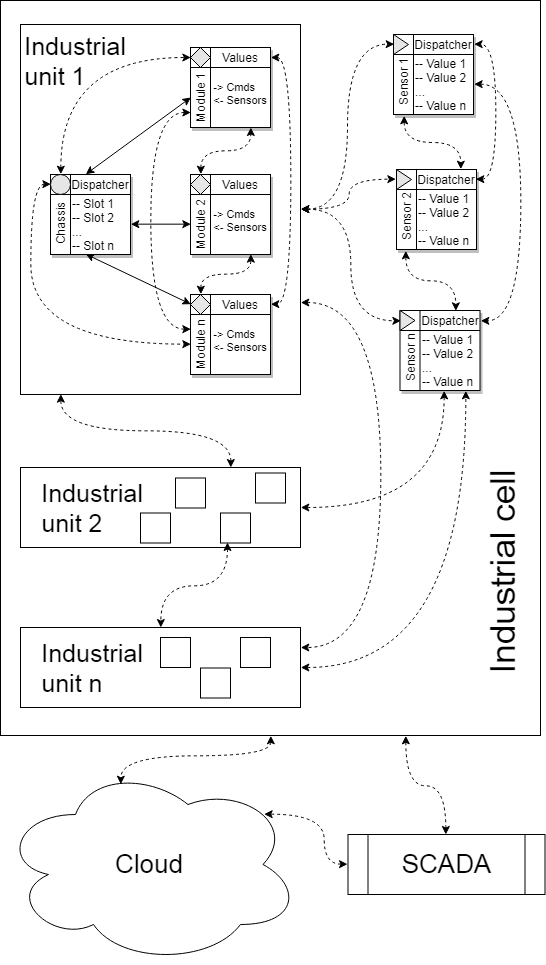
\includegraphics [width = 0.5 \textwidth]{ch-3/main-arch}
}
\caption *{Figure 1---Slot model of modular equipment} \label{fig: main-arch}
\end{figure}

The following procedure is proposed for initializing modules when they are connected to the dispatcher. The physical connection of each module is realized in three wires water interface, where the supply voltage is transmitted along two conductors, and the third is used as a safety line. The safety line unites all modules of one piece of equipment according to the wiring I. In this scheme, the safety line is pulled up by a resistor to the positive power supply. Since the resistance between line and ground is infinite, and between the supply and the line is equal to the value of the resistor, the voltage on the line is equal to the supply voltage. That is, a high level or logical one. As mentioned above, all modules are connected to the line and can short it to ground. Accordingly, the line will be at a high level if and only if all modules set a high level at their outputs. As soon as any of the modules connects the line to the ground, it will set a logic low level and no one module will be able to influence this.

The newly connected module first connects to the OpenThread network, then moves the security line to a logic low. The dispatcher detects this, after which it receives a list of all nodes closest to it (neighbors in OpenThread terminology), selects those that have the not connected status among them, and then asks the first of them to move the line back to a high logical level. If the level has changed, then the dispatcher and the module are connected to the same line, therefore, the module can be registered in the registry. Otherwise, the dispatcher moves to the next module in the list.

Since the main structure of storing and transmitting data in the system is JSON, the following describes a method for determining the maximum throughput of a data transmission channel when transmitting data in a given format through message queues. The following network scenarios are considered:

\begin{enumerate}
\item Interaction between operating system processes
\item Interaction of hardware and software modules in a heterogeneous computer network
\item Interaction with the user (operator)
\end{enumerate}

The experiments carried out are described below. The test equipment was a general-purpose personal computer (General PC), a laptop computer (Laptop), a high-performance server (server), a cloud virtual server (Virtual server) and an embedded system (Microcomputer). It is noted that the experiments carried out the transmission of JSON messages in a binary format. The following JSON binarization software libraries participated in the experiment: MessagePack, BSON, UBJSON, CBOR. The nanomsg software library was used as a message queue.

First, a comparison was made between TCP and UNIX socket throughput. It was noted that according to the results of measurements, the best way of interprocess communication in POSIX-compatible operating systems is TCP sockets. Next, we measured the average bandwidth of network connections. This part of the experiment showed that the use of the HTTP protocol leads to additional overhead costs, therefore this method is excluded from the calculation of the average throughput. Then the performance of the binary JSON packers was evaluated. It was noted that for all libraries there was practically no dependence of the compression ratio on the size of the JSON file. Then the dependence of the packing/unpacking speed on the size of the JSON file was obtained. of the reviewed libraries, this dependency is linear.The CBOR library showed the best time for both packing and unpacking.
The next step was to test the performance of CBOR libraries written in different programming languages. 1000 packing/unpacking cycles took place; the size of the original JSON file was 15 MB. Next, we measured the throughput of the nanomsg protocol.

Based on the data obtained, an overall performance evaluation of the message queue protocol was made. For this, the following formula is proposed (1):

\begin{equation}
\begin{split}
\label{eq: example}
\mathcal{B} _a = \frac{\mathcal{M}}{t}
= \frac{\mathcal{M}}{t_p + t_t + t_u}
= \frac{\mathcal{M}}
{\mathcal{M}/\mathcal{S} _p +
	\gamma \mathcal{M}/\mathcal{B} _t +
	\mathcal{M}/\mathcal{S} _u} = \\
= \frac{\mathcal{M}}
{\frac{\mathcal{M} _ (\mathcal{B} _t \mathcal{S} _u) +
		\gamma
		\mathcal{M} (\mathcal{S} _p \mathcal{S} _u) +
		\mathcal{M} (\mathcal{S} _p \mathcal{B} _t)}
	{\mathcal{S} _p \mathcal{B} _t \mathcal{S} _u}
}
= \frac{\mathcal{S} _p \mathcal{B} _t \mathcal{S} _u}
{\mathcal{B} _t \mathcal{S} _u + \gamma \mathcal{S} _p \mathcal{S} _u + \mathcal{S} _p \mathcal{B} _t} \,,
\end{split}
\end{equation}

\noindent where ${\mathcal{M}}$ is message size, $t$ is total time between two points, $t_p$ is packing time, $t_t$ is time transfer, $t_u$ is unpacking time, $\mathcal{S} _p$ is JSON data packing speed, $\mathcal{S} _u$ is JSON data unpacking speed, $\mathcal{ B} _t$ is message queue throughput, $\gamma$ is JSON compression ratio.

Python libraries often demonstrate performance, for example equal to the performance of the C libraries. This is because these libraries are simply wrappers for the C libraries. In this case, the use of the Python libraries is preferable because of the simpler syntax of the Python programming language. However, the Python libraries under consideration did not show sufficient performance, so it is obvious that the C library was chosen to implement the server side. When implementing the client side, the JS library was used, since this is the only option for implementing programs in the browser.

Table~1 shows the calculation results. Calculations show that the average bandwidth of the described communication channel ranges from \SI{6}{\percent} (worst case, packing/unpacking is required at both endpoints) to \SI{145}{\percent} (best case, no packing/unpacking is required at all, both endpoints use binary JSON data, which implies the ability to compress messages due to the fact that binary JSON takes up less space than plain JSON).

\begin{table}[!htb]
\centering
\caption *{Table 1---Bandwidth, cable connection, $\gamma=0.65$}
\label{tab: res}
\begin{IEEEeqnarraybox} [\IEEEeqnarraystrutmode \IEEEeqnarraystrutsizeadd{2pt}{0pt}]{x/u/Vx/r/v/r/v/r/x/}
\IEEEeqnarraydblrulerowcut \\

& \hfill% \raisebox{0pt} [0pt] [0pt]{Ratio$\mathcal{S} _u/\mathcal{S}$}
\hfill && \IEEEeqnarraymulticol{0}{h}{}%
\IEEEeqnarraystrutsize{0pt}{0pt} \\

&&&& \hfill \raisebox{0pt} [0pt] [0pt]{JS Library} \hfill &&
\hfill \raisebox{0pt} [0pt] [0pt]{C Library} \hfill &&
\hfill \raisebox{0pt} [0pt] [0pt]{Without unpacking} \hfill &
\IEEEeqnarraystrutsizeadd{0pt}{2pt} \\
%
\IEEEeqnarraydblrulerowcut \\

& JS Library &&& n/a \rlap{\textsuperscript{1}} &&{57.06} && 70.94 & \\
& &&& &&{(6.22 \, \%)} && (7.60 \, \%) & \\

& Library C &&& 67.50 && 117.70 && 203.18 & \\
& &&& (7.24 \, \%) && (12.62 \, \%) && (21.78 \, \%) & \\

& Unpacked &&& 93.31 && 227.27 &&{1354.98} & \\
& &&& (10.00 \, \%) && (24.37 \, \%) &&{(145.28 \, \%)} & \\
%
\IEEEeqnarraydblrulerowcut \\
& \IEEEeqnarraymulticol{9}{s}{\scriptsize \textsuperscript{1} Communication between clients is not implemented in this scenario.}%
\end{IEEEeqnarraybox}
\end{table}

Further in the chapter, it is noted that the bottleneck in the considered information model is the transmission of data over a wireless channel in an industrial environment. Therefore, a methodology for assessing the quality of the connection when using wireless communication modules is considered, in particular, the influence of industrial environment factors that can lead to a deterioration in communication is estimated. It is noted that testing will be carried out in the \SI{2.4}{\giga \hertz} frequency range, since this range is the most common in consumer data transmission networks: Wi-fi, Bluetooth, etc.

It is noted that the RSSI parameter is taken as the metric of the quality of the transmitted signal, since obtaining this parameter does not require the use of special measuring equipment (spectrum analyzers). Moreover, in the vast majority of consumer radio modules designed for the \SI{2.4}{\giga \hertz} frequency, this parameter is calculated automatically. It is also proposed to use an additional $RSSI_T$ metric based on antenna characteristics, taking into account antenna properties and signal attenuation~\cref{eq-1, eq-2, eq-3}:

\begin{equation}
RSSI_T = A-10 \mu \log (d),
\label{eq-1}
\end{equation}

\noindent where $d$ is the distance from the source, m; $\mu$ is the attenuation index, $\mu = 2$;

\begin{equation}
A = P_{out} + G_{tx} + G_{rx} -FSPL,
\label{eq-2}
\end{equation}

\noindent where $P_{out}$ is transmitter output power, dBm; $G_{tx}$ is gain of the original antenna, dBi; $G_{rx}$ is receiver antenna gain, dBi; $FSPL$ is path loss in free space, dB;

\begin{equation}
FSPL = 10\log(d) +20 \log (f) +20 \log (4 \pi/c),
\label{eq-3}
\end{equation}

\noindent where $f$ is frequency, Hz; $c = 299792458$ m/s.

Therefore, the proposed method uses the deviation$\Delta RSSI$, obtained as the difference between the measured value of $RSSI_P$ and the theoretical value of $RSSI_T$~\cref{eq-4}.

\begin{equation}
\Delta RSSI = RSSI_T-RSSI_P
\label{eq-4}
\end{equation}

Further, a hypothesis is put forward that if, when designing a wireless network, the location of nodes in a room is first determined, then it is logical to move from the $\Delta RSSI$ metric to the maximum distance between nodes~$D_{max}$~\cref{eq-5 }, a more convenient parameter for the problem under consideration. A signal with an RSSI value less than~-80 \, dBm is considered weak. Based on this hypothesis and~\cref{eq-4}, it is possible to calculate the $RSSI_T$ metric~\cref{eq-6} at a certain distance from the transmitter, taking into account the average deviation $\Delta RSSI$, which is influenced by factors of a specific production environment~\cref{eq-7}.

\begin{equation}
D_{max} = 10 ^ \frac{A-RSSI_T}{10 \mu}
\label{eq-5}
\end{equation}

\begin{equation}
RssI_T = -80- \overline{{\mathit \Delta} RSSI}
\label{eq-6}
\end{equation}

\begin{equation}
\overline{{\mathit \Delta} RSSI} = \frac1n \sum _{\substack{0 <i <n}}{\mathit \Delta} RSSI_i,
\label{eq-7}
\end{equation}

\noindent where $n$ is the number of dimensions. In this case $n = 25$.

The following describes a series of experiments carried out in real production conditions. An nRF52840 chip was used as a radio module, measurements were taken for various factors affecting the signal. Based on the results of the experiments, it was concluded that many production factors have a significant impact on the signal quality in the wireless network. However, the impact is not large enough to abandon the use of this technology. Moreover, the influence of many factors can be reduced through the use of a mesh topology and dense arrangement of receivers and transmitters. The importance of making appropriate measurements for each specific production facility is emphasized, as this ensures efficient placement of receivers and transmitters in production areas. It is also pointed out that the obtained results are especially interesting in the context of digitalization of production, where the wireless method of transmitting data from sensors is becoming preferable to the wired one due to the requirements for flexibility and mobility of the production process.


\textbf{The fourth chapter} describes the process of implementation of a modular platform for technological equipment. It is postulated that the modular technological platform (abbreviated~\textit{MTP}) is an experimental complex built on the basis of the approaches and techniques described in the previous chapters. The areas of application of such modular equipment are described, in particular, scenarios of application in small-scale and one-off production are considered. Further, the design features of the MTP are considered. It is shown that it structurally consists of a universal chassis~(abbreviated~\textit{USh}), which is equipped with coordinate tables with a carriage, on the suspension of which replaceable modules are placed.

Various designs are considered that can be used to create a UH. On the basis of a comparative analysis, the use of a Cartesian platform with a movable portal that implements movement in the XY plane is proposed as the basic chassis design. At the same time, it is noted that for many types of equipment that can be implemented on the basis of the MTP, an additional Z coordinate is not required, therefore, this coordinate in the MTP is optional and can be set if necessary.

Further, the analysis of existing drives is carried out, which can be used to create the US. Such types of linear drives are considered as a linear stepper motor, chain transmission, gears based on toothed belts, as well as ball-screw and roller-screw drives. Also, various types of guides along which linear movement will be carried out are considered, in particular, options with rail guides of various types and guides based on smooth cylindrical shafts are considered. On the basis of a comparative analysis of the advantages and disadvantages of all the considered solutions, the use of ball screw drives with smooth cylindrical guides is proposed as a design of linear drives for USh.

After choosing the design of linear drives, an analysis of existing electric motors is provided, two main types of electric motors are considered: geared servo motors and stepper motors. A number of comparison criteria are highlighted, according to the results of which preference is given to stepper motors. The next step is to describe the final electro-kinematic diagram of the USh~coordinate table (Figure~2).

\begin{figure} [ht]
\centerfloat{
	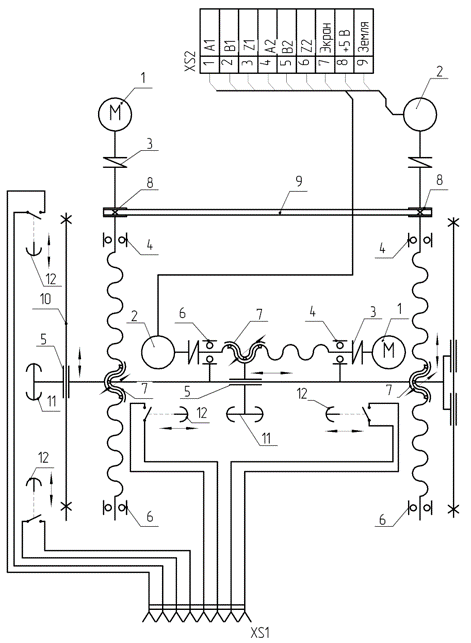
\includegraphics [width=0.7\textwidth]{ch-4/el-mech-sch}
}
\caption *{Figure 2---Electrokinematic diagram of the coordinate table: 1---stepping motor, 2---rotation angle sensor, 3---cam clutch, 4---Radial bearing, 5---linear bearing, 6---Radial bearing, 7---Ball screw, 8---Toothed pulley, 9---Toothed belt, 10---Guide, 11---Slotted optical sensor, 12---Limit switch} \label{fig: scheme}
\end{figure}

The final section of the chapter is devoted to the description of the development of the universal control unit for USh. The USH is the central component of the MTP, since it allows you to connect the hardware part of the equipment created on the basis of this concept (it receives data from the USH sensors and working bodies, generates control signals of the drives) and the software part (connects the equipment with a PC and allows two-way data exchange with the MTP). The universal control unit consists of the following modules:

\begin{itemize}
\item Power module.
\item Processor module.
\item PC interface module.
\item Sensor interface module.
\item Drive control modules.
\item Module of indication and interaction with the operator.
\end{itemize}

All modules will have their own microkontroller, providing their interaction under the SPI protocol \footnote{abbr.~from~eng. English \textit{Serial Peripheral Interface, SPI bus.}---serial peripheral interface, SPI bus.} This protocol will allow all modules to communicate with each other and exchange the necessary information in a synchronous serial mode. That is, the universal control unit is a network of microcontrollers, providing various functions .

\FloatBarrier                      
\textbf{In conclusion}, the main results of the work are given, which are as follows:
%% Согласно ГОСТ Р 7.0.11-2011:
%% 5.3.3 В заключении диссертации излагают итоги выполненного исследования, рекомендации, перспективы дальнейшей разработки темы.
%% 9.2.3 В заключении автореферата диссертации излагают итоги данного исследования, рекомендации и перспективы дальнейшей разработки темы.

The significance of the results obtained in the dissertation work is emphasized by the possibility of integrating the developed methods, approaches, and algorithms into the computer-aided design system of modular technological equipment. The proposed recommendations for the creation of units and assemblies and control units for modular technological equipment will simplify its development and use in the conditions of single and small-scale production. During the research, the following main theoretical and practical results were obtained:

\begin{enumerate}
\item A universal design of re-adjustable modular equipment is proposed, consisting of a universal coordinate chassis with a movable carriage; modules that determine the main operation performed by the equipment and are installed on the suspension of the chassis carriage using an electromagnetic fastening; and a modular control unit that implements a numerical control algorithm.
\item Algorithmic and software and hardware support for the modular control unit has been developed, which includes a set of software and hardware tools for implementing decentralized network interaction of modules and software for automatic reconfiguration of a unit of modular equipment, which reduces the complexity of the changeover.
\item A method for unifying modules with an electromagnetic mount has been developed, which includes a method for determining the parameters of unification and their limitations and a method for forming a parametric series based on the formulated limitations.
\item A criterion for the expediency of using modular equipment is proposed, based on the analysis of group technological processes, making it possible to assess the prospects for using modular equipment for typical technological processes used at an enterprise.
\item A method for optimizing a set of modular equipment has been developed, which includes a method for calculating the weight coefficients of the optimization objective function and a two-criterion optimization algorithm based on the theory of normalization and the discrete-event method.
\item Based on the methodology for optimizing a set of modular equipment, software was developed, and a numerical experiment was carried out, which showed an increase in the productivity of a group of products by~\SI{18}{\percent}.
\item To test the proposed design of modular equipment and methods and algorithms for working with it, a prototype of a modular technological platform was created.
\end{enumerate}

Thus, based on the results obtained, the goal of this dissertation research on the development of methods for the design and use of modular technological equipment in the conditions of single and small-scale production can be considered achieved.

The results obtained correspond to paragraph 6 ``Development, research and implementation of new types of technological equipment for the manufacture of parts, assembly, adjustment, control and testing of devices'' and paragraph 7 ``development and implementation of new methods and means of mechanization, automation, robotization of instrument-making production, providing an increase in productivity, a decrease in labor intensity and an increase in the efficiency of production'' specialty passport 05.11.14---`` Instrument-making technology''.


\ifdefmacro{\microtypesetup}{\microtypesetup{protrusion=false}}{} % не рекомендуется применять пакет микротипографики к автоматически генерируемому списку литературы
\urlstyle{rm}                               % ссылки URL обычным шрифтом
\ifnumequal{\value{bibliosel}}{0}{% Встроенная реализация с загрузкой файла через движок bibtex8
  \renewcommand{\bibname}{\large \bibtitleauthor}
  \nocite{*}
  \insertbiblioauthor           % Подключаем Bib-базы
  %\insertbiblioexternal   % !!! bibtex не умеет работать с несколькими библиографиями !!!
}{% Реализация пакетом biblatex через движок biber
  % Цитирования.
  %  * Порядок перечисления определяет порядок в библиографии (только внутри подраздела, если `\insertbiblioauthorgrouped`).
  %  * Если не соблюдать порядок "как для \printbibliography", нумерация в `\insertbiblioauthor` будет кривой.
  %  * Если цитировать каждый источник отдельной командой --- найти некоторые ошибки будет проще.
  %
  %% authorconf
  \nocite{confbib-2017-trajectory-problems}%
  \nocite{confbib-2017-json}%
  \nocite{confbib-2017-modular-integration}%
  \nocite{confbib-2017-machine-vision}%
  \nocite{confbib-2017-microservices}%
  \nocite{confbib-2018-motion-profile}%
  \nocite{confbib-2018-etherium}%
  \nocite{confbib-2018-mesh}%
  \nocite{confbib-2018-blockchain}%
  \nocite{confbib-2019-interpolation}%
  \nocite{confbib-2019-voice-assistant}%
  \nocite{vakbib-wpan-2020}%
  \nocite{confbib-2020-smart-controller}%
  \nocite{confbib-2020-auto-positioning}%
  \nocite{confbib-2020-RSSI}
  %
  %% authorvak
  \nocite{vakbib-microservice-2018}%
  \nocite{vakbib-blockchain-2019}%
  \nocite{vakbib-machine-vision-2020}%
  %
  %% authorwos
  %\nocite{wosbib1}%
  %
  %% authorscopus
  %\nocite{scbib1}%
  %
  %% authorpathent
  %\nocite{patbib1}%
  %
  %% authorprogram
  %\nocite{progbib1}%
  %
  %% authorother
  %\nocite{bib1}%
  %\nocite{bib2}%

  \ifnumgreater{\value{usefootcite}}{0}{
    \begin{refcontext}[labelprefix={}]
      \ifnum \value{bibgrouped}>0
        \insertbiblioauthorgroupedEn    % Вывод всех работ автора, сгруппированных по источникам
      \else
        \insertbiblioauthor      % Вывод всех работ автора
      \fi
    \end{refcontext}
  }{
  \ifnum \totvalue{citeexternal}>0
    \begin{refcontext}[labelprefix=A]
      \ifnum \value{bibgrouped}>0
        \insertbiblioauthorgroupedEn    % Вывод всех работ автора, сгруппированных по источникам
      \else
        \insertbiblioauthor      % Вывод всех работ автора
      \fi
    \end{refcontext}
  \else
    \ifnum \value{bibgrouped}>0
      \insertbiblioauthorgroupedEn    % Вывод всех работ автора, сгруппированных по источникам
    \else
      \insertbiblioauthor      % Вывод всех работ автора
    \fi
  \fi
  %  \insertbiblioauthorimportant  % Вывод наиболее значимых работ автора (определяется в файле characteristic во второй section)
  \begin{refcontext}[labelprefix={}]
      \insertbiblioexternal            % Вывод списка литературы, на которую ссылались в тексте автореферата
  \end{refcontext}
  % Невидимый библиографический список для подсчёта количества внешних публикаций
  % Используется, чтобы убрать приставку "А" у работ автора, если в автореферате нет
  % цитирований внешних источников.
  \printbibliography[heading=nobibheading, section=0, env=countexternal, keyword=biblioexternal, resetnumbers=true]%
  }
}
\ifdefmacro{\microtypesetup}{\microtypesetup{protrusion=true}}{}
\urlstyle{tt}                               % возвращаем установки шрифта ссылок URL
